\documentclass[tikz,border=8pt]{standalone}
\begin{document}
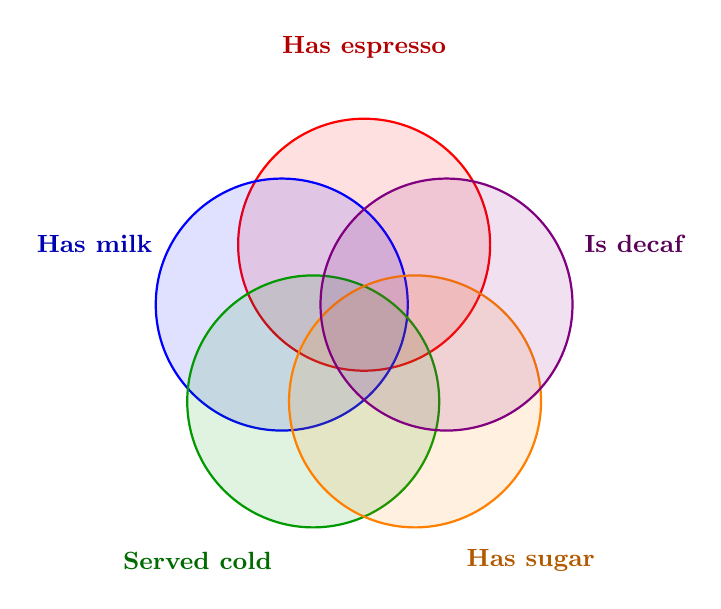
\begin{tikzpicture}
\def\d{1.1}\def\r{1.6}
\foreach \i/\n/\c/\a in {0/Has espresso/red/90,1/Has milk/blue/162,2/Served cold/green!60!black/234,3/Has sugar/orange/306,4/Is decaf/violet/18}{
 \draw[\c,thick,fill=\c,fill opacity=0.12] (\a:\d) circle (\r);
 \node[\c!70!black,font=\small\bfseries,align=center] at (\a:{\d+\r+0.9}) {\n};
}
\end{tikzpicture}
\end{document}
